% !TEX root = main.tex

\section{简介}

\subsection{实验目的}

\begin{itemize}[noitemsep]
    \item 熟悉x86-64架构汇编语言.
    \item 掌握二进制调试器的使用.
    \item 学习反汇编与逆向工程方法.
\end{itemize}

\subsection{实验要求}

使用 \verb|objdump|、\verb|gdb|、\verb|strings| 等工具, 通过反汇编与逆向工程方法, 分析可执行文件 \verb|bomb| 的工作原理, 破解该程序要求输入的若干不同字符串, 从而拆除“二进制炸弹”. \par
该二进制炸弹共分7个关卡(含1个隐藏关卡).

\subsection{实验环境}

\def\envcontent{本实验需要在x86-64环境下用gdb调试glibc程序. 由于笔者的MacBook为ARM架构, 最初计划在Docker容器中部署完整Linux实验环境(参见Data Lab实验报告). 调查发现, 用于仿真x86-64架构的QEMU并未实现ptrace, 无法直接在容器内调试, 仅支持一种在主机上运行gdb并远程连接的调试方法(详细描述转见issue: \url{https://github.com/docker/for-mac/issues/5191} 及QEMU官方文档: \url{https://qemu.readthedocs.io/en/latest/system/gdb.html}). 然而, 在基于ARM的Mac机器上安装gdb并非常规做法, 缺乏良好支持. 笔者决定放弃远程调试的方案, 转移到原生x86-64的机器下进行本实验.}

本实验所有命令均在以下环境执行\footnote{\envcontent}:
\vspace{8pt}\par{\small\begin{tabular}{ll}
    Machine & ASUS FH5900V Notebook PC\\
    Processor & Intel(R) Core(TM) i7-6700HQ CPU @ 2.60Hz \\
    Memory & 4GB DDR4 2133MHz \\
    System & Windows 10家庭中文版, 64位, 基于x64 \\
    WSL Distro & Ubuntu 20.04.4 LTS \\
    Packages & GNU Binutils 2.34, GDB 9.2.0
\end{tabular}}

\begin{figure}[H]
    \centering
    \includegraphics[width=0.85\textwidth]{env.png}
    \caption{在WSL中运行gdb}\label{fig:env}
\end{figure}

\section{实验成果}

\begin{figure}[H]
    \centering
    \includegraphics[width=\textwidth]{ans.png}
    \caption{在WSL中拆除炸弹}
\end{figure}

\section{实验过程}\label{procedure}

\subsection{准备工作}\label{prepare}

根据实验材料中的提示, 首先利用GNU Binutils提供的 \verb|objdump| 工具反汇编 \verb|bomb| 文件. 在工作路径中执行命令
\begin{code}{text}
    $ objdump -d bomb > disas.txt
\end{code}
从而将结果存入 \verb|disas.txt| 中, 以备后续参阅. 输出包括了  \verb|.init|, \verb|.plt|, \verb|.text|, \verb|.fini| 等4个节的反汇编结果, 涵盖了主要的机器指令. 输出还注明了文件格式为 \verb|elf64-x86-64|, 因此可使用 \verb|readelf| 工具查看该文件头信息
\begin{code}{text}
    $ readelf -h bomb
\end{code}
有如下结果
\begin{code}{text}
ELF Header:
  Magic:   7f 45 4c 46 02 01 01 00 00 00 00 00 00 00 00 00
  Class:                             ELF64
  Data:                              2's complement, little endian
  Version:                           1 (current)
  OS/ABI:                            UNIX - System V
  ABI Version:                       0
  Type:                              EXEC (Executable file)
  Machine:                           Advanced Micro Devices X86-64
  Version:                           0x1
  Entry point address:               0x400c90
  Start of program headers:          64 (bytes into file)
  Start of section headers:          18616 (bytes into file)
  Flags:                             0x0
  Size of this header:               64 (bytes)
  Size of program headers:           56 (bytes)
  Number of program headers:         9
  Size of section headers:           64 (bytes)
  Number of section headers:         36
  Section header string table index: 33
\end{code}
可见, 该ELF文件采用小端格式补码表示数据, 依赖于Unix的二进制接口, 需在x86-64机器中运行. 映证了搭建相应实验环境的必要性. 
上述结果还指出程序入口点地址为 \verb|0x400c90|, 即 \verb|.text| 节的起始地址. 

自然地想到用 \verb|nm| 工具打印代码段的符号
\begin{code}{text}
    $ nm bomb | grep -w T | sort > syms.txt
\end{code}
得到按地址升序排列的结果, 见附录 \nameref{syms}.
其中包括了 \verb|bomb.c| 中出现的函数名, 如 \verb|main|, \verb|phase_defused| 等. 也包括了被隐藏的函数名, 如 \verb|secret_phase|, \verb|read_six_numbers| 等. 显然, 该二进制炸弹有隐藏关卡.

另一方面, 根据提示, 可以使用 \verb|strings| 工具打印 \verb|bomb| 文件中所有字符串. 此处我们使用 \verb|readelf| 工具, 以字符串形式导出 \verb|.rodata| 节的内容
\begin{code}{text}
    $ readelf -p .rodata bomb > rodata.txt
\end{code}
结果见附录 \nameref{rodata}.
观察发现, 其中用于交互或报错的居多, 部分串在 \verb|bomb.c| 文件中直接出现. 而“Border relations with Canada have never been better.”“flyers”等串较为突兀, 应当引起注意.

下面, 利用 \verb|gdb| 工具逐关卡破解炸弹程序. 进入gdb并载入bomb文件, 应有如图 \ref{fig:env} 所示输入输出. 在各关卡的入口处设置断点, 以防炸弹爆炸
\begin{code}{text}
(gdb) break phase_1
Breakpoint 1 at 0x400ee0
(gdb) break phase_2
Breakpoint 2 at 0x400efc
(gdb) break phase_3
Breakpoint 3 at 0x400f43
(gdb) break phase_4
Breakpoint 4 at 0x40100c
(gdb) break phase_5
Breakpoint 5 at 0x401062
(gdb) break phase_6
Breakpoint 6 at 0x4010f4
(gdb) break secret_phase
Breakpoint 7 at 0x401242
\end{code}

\subsection{\texttt{phase_1}}

运行程序, 输入任意字符串, 触发 \verb|phase_1| 处断点, 进而反汇编当前函数
\begin{code}{text}
(gdb) run
Starting program: /home/hasined/Repositories/Computer-System/labs/bomb/bomb/bomb
Welcome to my fiendish little bomb. You have 6 phases with
which to blow yourself up. Have a nice day!
My ID is PB20061372

Breakpoint 1, 0x0000000000400ee0 in phase_1 ()
(gdb) disas
Dump of assembler code for function phase_1:
=> 0x0000000000400ee0 <+0>:     sub    $0x8,%rsp
   0x0000000000400ee4 <+4>:     mov    $0x402400,%esi
   0x0000000000400ee9 <+9>:     callq  0x401338 <strings_not_equal>
   0x0000000000400eee <+14>:    test   %eax,%eax
   0x0000000000400ef0 <+16>:    je     0x400ef7 <phase_1+23>
   0x0000000000400ef2 <+18>:    callq  0x40143a <explode_bomb>
   0x0000000000400ef7 <+23>:    add    $0x8,%rsp
   0x0000000000400efb <+27>:    retq
End of assembler dump.
\end{code}
分析汇编代码主体部分, 得知大意为:

\begin{enumerate}[noitemsep]
    \item 将 \verb|0x402400| 移入 \verb|esi| 中.
    \item 调用 \verb|strings_not_equal|.
    \item 若 \verb|eax| 为0, 跳转至函数尾部; 否则调用 \verb|explode_bomb|.
\end{enumerate}
显然, \verb|explode_bomb| 为实现炸弹爆炸的函数. 出于安全起见,
在该函数入口设置断点
\begin{code}{text}
(gdb) break explode_bomb
Breakpoint 8 at 0x40143a
\end{code}
从而在后续实验过程中避免非预期的爆炸.

根据代码逻辑, 在 \verb|0x400eee| 处设置断点, 程序运行到此处时修改 \verb|eax| 为0, 即可通过 \verb|phase_1| . 输入输出如下

\begin{code}{text}
(gdb) break *0x400eee
Breakpoint 9 at 0x400eee
(gdb) continue
Continuing.

Breakpoint 9, 0x0000000000400eee in phase_1 ()
(gdb) set $eax=0
(gdb) continue
Continuing.
Phase 1 defused. How about the next one?
\end{code}
每个关卡都可以用修改寄存器值的手段作弊通过, 往后不再使用类似方法, 而是以正常途径得出答案.

合理猜测, \verb|strings_not_equal| 函数用于比较两字符串, 两字符串相等时返回0. 结合x86-64 System V的调用习惯, 可知作为实参的字符串指针有一个位于 \verb|esi| 中, 此处传入 \verb|0x402400|; 另一指针应当位于 \verb|edi| 或 \verb|rdi| 中; 返回值存于 \verb|eax| 中. 

出于验证目的, 可以将被调函数 \verb|strings_not_equal| 反汇编
\begin{code}{text}
    (gdb) disas strings_not_equal
\end{code}
或者在\nameref{prepare}的 \texttt{disas.txt} 文件中查找, 往后不再特别指出. 由汇编代码\footnote{见附录 \nameref{strings-not-equal}}, 可知函数逻辑
\begin{enumerate}[noitemsep]
    \item 调用 \verb|string_length|, 分别得到 \verb|rdi|, \verb|rsi| 中字符串的长度.
    \item 比较两字符串长度, 若不相等, 返回1.
    \item 逐个比较每一位, 若不相等, 返回1; 否则返回0.
\end{enumerate}
与假设相符. 为了确认实参 \verb|rdi| 的含义, 将 \verb|main| 函数反汇编, 发现在调用 \verb|phase_1| 前有如下语句
\begin{code}{text}
    0x0000000000400e32 <+146>:   callq  0x40149e <read_line>
    0x0000000000400e37 <+151>:   mov    %rax,%rdi
\end{code}
对应到 \texttt{bomb.c} 中为
\begin{code}{c}
    input = read_line();             /* Get input                   */
    phase_1(input);                  /* Run the phase               */    
\end{code}
可知 \verb|rdi| 存入了 \verb|read_line| 函数的返回值, 即所输入字符串的指针. 

至此, \verb|phase_1| 得到解决. 该关卡要求输入的字符串与 \verb|0x402400| 指向的字符串严格相等. 检查得到答案
\begin{code}{text}
(gdb) x/s 0x402400
0x402400:       "Border relations with Canada have never been better."
\end{code}
重新运行程序并输入“Border relations with Canada have never been better.”, 成功通过 \verb|phase_1|. 输入输出如下
\begin{code}{text}
(gdb) disable 1
(gdb) disable 9
(gdb) run
The program being debugged has been started already.
Start it from the beginning? (y or n) y
Starting program: /home/hasined/Repositories/Computer-System/labs/bomb/bomb/bomb
Welcome to my fiendish little bomb. You have 6 phases with
which to blow yourself up. Have a nice day!
Border relations with Canada have never been better.
Phase 1 defused. How about the next one?
\end{code}
事实上, 在\nameref{prepare}的 \nameref{rodata} 中已经找到了答案.

\subsection{\texttt{phase_2}}

来到 \verb|phase_2| 的断点处并反汇编
\begin{code}{text}
Breakpoint 2, 0x0000000000400efc in phase_2 ()
(gdb) disas
Dump of assembler code for function phase_2:
=> 0x0000000000400efc <+0>:     push   %rbp
   0x0000000000400efd <+1>:     push   %rbx
   0x0000000000400efe <+2>:     sub    $0x28,%rsp
   0x0000000000400f02 <+6>:     mov    %rsp,%rsi
   0x0000000000400f05 <+9>:     callq  0x40145c <read_six_numbers>
   ...                          ...    ...
   0x0000000000400f3c <+64>:    add    $0x28,%rsp
   0x0000000000400f40 <+68>:    pop    %rbx
   0x0000000000400f41 <+69>:    pop    %rbp
   0x0000000000400f42 <+70>:    retq
End of assembler dump.
\end{code}
发现该关卡以栈帧顶部指针为参数, 调用 \verb|read_six_numbers|. 合理猜测, 该函数从输入字符串读出6个数字并返回到栈帧中. 出于验证目的, 将其反汇编\footnote{见附录 \nameref{read-six-numbers}}, 梳理得其功能为
\begin{enumerate}[noitemsep]
    \item 调用动态链接的 \verb|sscanf|, 传入的参数依次为: \verb|rdi|, \verb|0x4025c3|, \verb|rsi|, \verb|rsi+4|, \verb|rsi+8|, \verb|rsi+12|, \verb|rsi+16|, \verb|rsi+20|.
    \item 若 \verb|sscanf| 的返回值 \verb|eax| 不大于5, 调用 \verb|explode_bomb|, 否则跳转至函数尾部.
\end{enumerate}
应当注意, \verb|sscanf| 的前6个参数通过寄存器传递, 而后2个参数通过栈帧传递. \verb|sscanf| 是用于格式化输入数据的标准库函数, 在此处, 作为输入源的字符串由 \verb|read_line| 获得, 作为格式控制的字符串位于地址 \verb|0x4025c3|, 可用gdb查看
\begin{code}{text}
    (gdb) x/s 0x4025c3
    "%d %d %d %d %d %d"
\end{code}
返回的6个整数位于 \verb|phase_2| 函数的栈帧中, 地址依次为\verb|rsp|, \verb|rsp+4|, \verb|rsp+8|, \verb|rsp+12|, \verb|rsp+16| 和 \verb|rsp+20|. 若输入字符串所含整数少于6个, 炸弹爆炸. 

省略号部分的汇编代码如下
\begin{code}{text}
   0x0000000000400f0a <+14>:    cmpl   $0x1,(%rsp)
   0x0000000000400f0e <+18>:    je     0x400f30 <phase_2+52>
   0x0000000000400f10 <+20>:    callq  0x40143a <explode_bomb>
   0x0000000000400f15 <+25>:    jmp    0x400f30 <phase_2+52>
   0x0000000000400f17 <+27>:    mov    -0x4(%rbx),%eax
   0x0000000000400f1a <+30>:    add    %eax,%eax
   0x0000000000400f1c <+32>:    cmp    %eax,(%rbx)
   0x0000000000400f1e <+34>:    je     0x400f25 <phase_2+41>
   0x0000000000400f20 <+36>:    callq  0x40143a <explode_bomb>
   0x0000000000400f25 <+41>:    add    $0x4,%rbx
   0x0000000000400f29 <+45>:    cmp    %rbp,%rbx
   0x0000000000400f2c <+48>:    jne    0x400f17 <phase_2+27>
   0x0000000000400f2e <+50>:    jmp    0x400f3c <phase_2+64>
   0x0000000000400f30 <+52>:    lea    0x4(%rsp),%rbx
   0x0000000000400f35 <+57>:    lea    0x18(%rsp),%rbp
   0x0000000000400f3a <+62>:    jmp    0x400f17 <phase_2+27>
\end{code}
其大意为
\begin{enumerate}[noitemsep]
    \item 若第1个整数不为1, 炸弹爆炸.
    \item 进入循环结构: 对每个$i=2,3,\cdots,6$, 若第$i$整数不是第$i-1$整数的2倍, 炸弹爆炸.
\end{enumerate}
故要求输入的6个整数为“1 2 4 8 16 32”. 

重新运行程序, 输入答案, 在 \verb|add $0x28,%rsp| 处设置断点
\begin{code}{text}
(gdb) break *0x400f3c
Breakpoint 10 at 0x400f3c
(gdb) continue
Continuing.

Breakpoint 10, 0x0000000000400f3c in phase_2 ()
(gdb) x/6wd $rsp
0x7fffffffdf60: 1       2       4       8
0x7fffffffdf70: 16      32
(gdb) continue
Continuing.
That's number 2.  Keep going!
\end{code}
顺利到达断点处, 并且栈帧中的数据与前面的分析相符.

\subsection{\texttt{phase_3}}

将 \verb|phase_3| 反汇编, 发现调用了 \verb|sscanf|, 代码结构与 \verb|read_six_numbers| 相似
\begin{code}{text}
Dump of assembler code for function phase_3:
=> 0x0000000000400f43 <+0>:     sub    $0x18,%rsp
   0x0000000000400f47 <+4>:     lea    0xc(%rsp),%rcx
   0x0000000000400f4c <+9>:     lea    0x8(%rsp),%rdx
   0x0000000000400f51 <+14>:    mov    $0x4025cf,%esi
   0x0000000000400f56 <+19>:    mov    $0x0,%eax
   0x0000000000400f5b <+24>:    callq  0x400bf0 <__isoc99_sscanf@plt>
   0x0000000000400f60 <+29>:    cmp    $0x1,%eax
   0x0000000000400f63 <+32>:    jg     0x400f6a <phase_3+39>
   0x0000000000400f65 <+34>:    callq  0x40143a <explode_bomb>
   ...                          ...    ...
   0x0000000000400fc9 <+134>:   add    $0x18,%rsp
   0x0000000000400fcd <+138>:   retq
End of assembler dump.
\end{code}
检查其格式, 发现要求输入2个整数
\begin{code}{text}
(gdb) x/s 0x4025cf
0x4025cf:       "%d %d"
\end{code}

目标是找出2个整数应当满足的条件. 观察省略号部分的代码, 发现有大量重复结构
\begin{code}{text}
   0x0000000000400f6a <+39>:    cmpl   $0x7,0x8(%rsp)
   0x0000000000400f6f <+44>:    ja     0x400fad <phase_3+106>
   0x0000000000400f71 <+46>:    mov    0x8(%rsp),%eax
   0x0000000000400f75 <+50>:    jmpq   *0x402470(,%rax,8)
   0x0000000000400f7c <+57>:    mov    $0xcf,%eax
   0x0000000000400f81 <+62>:    jmp    0x400fbe <phase_3+123>
   0x0000000000400f83 <+64>:    mov    $0x2c3,%eax
   0x0000000000400f88 <+69>:    jmp    0x400fbe <phase_3+123>
   0x0000000000400f8a <+71>:    mov    $0x100,%eax
   0x0000000000400f8f <+76>:    jmp    0x400fbe <phase_3+123>
   0x0000000000400f91 <+78>:    mov    $0x185,%eax
   0x0000000000400f96 <+83>:    jmp    0x400fbe <phase_3+123>
   0x0000000000400f98 <+85>:    mov    $0xce,%eax
   0x0000000000400f9d <+90>:    jmp    0x400fbe <phase_3+123>
   0x0000000000400f9f <+92>:    mov    $0x2aa,%eax
   0x0000000000400fa4 <+97>:    jmp    0x400fbe <phase_3+123>
   0x0000000000400fa6 <+99>:    mov    $0x147,%eax
   0x0000000000400fab <+104>:   jmp    0x400fbe <phase_3+123>
   0x0000000000400fad <+106>:   callq  0x40143a <explode_bomb>
   0x0000000000400fb2 <+111>:   mov    $0x0,%eax
   0x0000000000400fb7 <+116>:   jmp    0x400fbe <phase_3+123>
   0x0000000000400fb9 <+118>:   mov    $0x137,%eax
   0x0000000000400fbe <+123>:   cmp    0xc(%rsp),%eax
   0x0000000000400fc2 <+127>:   je     0x400fc9 <phase_3+134>
   0x0000000000400fc4 <+129>:   callq  0x40143a <explode_bomb>
\end{code}
其中使用间接比例变址寻址方式的 \verb|jmpq *0x402470(,%rax,8)| 一行值得重视. 加之紧随其后有大量相同的 \verb|jmp| 操作, 有充分的理由猜测这是 \verb|switch| 语句的编译结果. 

首先, 我们查看 \verb|0x402470| 指向的跳转表

\begin{code}{text}
(gdb) x/8g 0x402470
0x402470:       0x400f7c <phase_3+57>   0x400fb9 <phase_3+118>
0x402480:       0x400f83 <phase_3+64>   0x400f8a <phase_3+71>
0x402490:       0x400f91 <phase_3+78>   0x400f98 <phase_3+85>
0x4024a0:       0x400f9f <phase_3+92>   0x400fa6 <phase_3+99>
\end{code}
然后, 根据跳转结果, 将汇编代码翻译为C语言
\begin{code}{c}
    sscanf(input, "%d %d", &index, &number);
    switch (index) {
    case 0:
        eax = 207;      // mov 0xcf(%rsp),%eax
        break;          // jmp 0x400fbe <phase_3+123>
    case 1:
        eax = 311;      // mov 0x137(%rsp),%eax
        break;          
    case 2:
        eax = 707;      // mov 0x2c3(%rsp),%eax
        break;          // jmp 0x400fbe <phase_3+123>
    case 3:
        eax = 256;      // mov 0x100(%rsp),%eax
        break;          // jmp 0x400fbe <phase_3+123>
    case 4:
        eax = 389;      // mov 0x185(%rsp),%eax
        break;          // jmp 0x400fbe <phase_3+123>
    case 5:
        eax = 206;      // mov 0xce(%rsp),%eax
        break;          // jmp 0x400fbe <phase_3+123>
    case 6:
        eax = 682;      // mov 0x2aa(%rsp),%eax
        break;          // jmp 0x400fbe <phase_3+123>
    case 7:
        eax = 327;      // mov 0x147(%rsp),%eax
        break;          // jmp 0x400fbe <phase_3+123>
    default:
        explode_bomb(); eax = 0;
    }
    if (eax != number) explode_bomb();
\end{code}
其中, \verb|index|, \verb|number| 分别为  \verb|rsp+8|, \verb|rsp+12| 指向的整数, 两者应当满足的映射关系已十分显然: 当 \verb|index| = 0 时, \verb|number| 必须为 \verb|0xcf|, 即207; 当 \verb|index| = 1 时, \verb|number| = \verb|0x137|, 即311; 依此类推. 故本关卡共有8种可行的答案, 部分试验结果如下
\begin{code}{text}
(gdb) disable 3
(gdb) break *0x400e86
Breakpoint 11 at 0x400e86: file bomb.c, line 94.
(gdb) jump *0x400e5b
Continuing at 0x400e5b.
That's number 2.  Keep going!
0 207
Halfway there!

Breakpoint 11, main (argc=<optimized out>, argv=<optimized out>) at bomb.c:94
94          input = read_line();
(gdb) jump *0x400e5b
Continuing at 0x400e5b.
That's number 2.  Keep going!
1 311
Halfway there!

...

Breakpoint 11, main (argc=<optimized out>, argv=<optimized out>) at bomb.c:94
94          input = read_line();
(gdb) jump *0x400e5b
Continuing at 0x400e5b.
That's number 2.  Keep going!
7 327
Halfway there!
\end{code}

一个有趣的事实是, 在使用 \verb|jump| 命令反复试验的过程中, 炸弹提前输出了2次“Congratulations! You've defused the bomb!”

\subsection{\texttt{phase_4}}

将 \verb|phase_4| 反汇编
\begin{code}{text}
Dump of assembler code for function phase_4:
   0x000000000040100c <+0>:     sub    $0x18,%rsp
   0x0000000000401010 <+4>:     lea    0xc(%rsp),%rcx
   0x0000000000401015 <+9>:     lea    0x8(%rsp),%rdx
   0x000000000040101a <+14>:    mov    $0x4025cf,%esi
   0x000000000040101f <+19>:    mov    $0x0,%eax
   0x0000000000401024 <+24>:    callq  0x400bf0 <__isoc99_sscanf@plt>
   0x0000000000401029 <+29>:    cmp    $0x2,%eax
   0x000000000040102c <+32>:    jne    0x401035 <phase_4+41>
   0x000000000040102e <+34>:    cmpl   $0xe,0x8(%rsp)
   0x0000000000401033 <+39>:    jbe    0x40103a <phase_4+46>
   0x0000000000401035 <+41>:    callq  0x40143a <explode_bomb>
   ...                          ...    ...
   0x000000000040105d <+81>:    add    $0x18,%rsp
   0x0000000000401061 <+85>:    retq
End of assembler dump.
\end{code}
发现前6行与 \verb|phase_3| 完全一致, 同样都要求输入2个整数. 区别在于输入数据数目严格为2, 并且第1个无符号整数不得大于14.

省略号部分如下
\begin{code}{text}
   0x000000000040103a <+46>:    mov    $0xe,%edx
   0x000000000040103f <+51>:    mov    $0x0,%esi
   0x0000000000401044 <+56>:    mov    0x8(%rsp),%edi
   0x0000000000401048 <+60>:    callq  0x400fce <func4>
   0x000000000040104d <+65>:    test   %eax,%eax
   0x000000000040104f <+67>:    jne    0x401058 <phase_4+76>
   0x0000000000401051 <+69>:    cmpl   $0x0,0xc(%rsp)
   0x0000000000401056 <+74>:    je     0x40105d <phase_4+81>
   0x0000000000401058 <+76>:    callq  0x40143a <explode_bomb>
\end{code}
发现调用了名为 \verb|func4| 的函数, 传入的参数 \verb|edi|, \verb|esi|, \verb|edx| 分别为输入的第1个整数, 0 和 14. 若返回值不为0, 炸弹爆炸. 

根据最后3行, 输入的第2个整数必须为0. 因此本关卡可通过枚举第1个整数解决.

注意到 \verb|func4| 的汇编代码\footnote{见附录 \nameref{func4}}涉及递归, 为了清晰, 将其翻译为C语言进行分析. 
\begin{code}{c}
int func4(int edi, int esi, int edx) {
    int eax = edx - esi;
    eax += eax >> 31;
    eax >>= 1;
    int ecx = esi + eax;
    if (edi < ecx)
        return func4(edi, esi, ecx - 1) * 2;
    else if (edi > ecx)
        return func4(edi, ecx + 1, edx) * 2 + 1;
    else
        return 0;
}
\end{code}
类似于二分查找, 但似乎逻辑更为复杂. 稍加分析, 知 \verb|eax += eax >> 31| 与 \verb|eax >>= 1| 两句实为C语言整数除法 \verb|eax /= 2| 的编译结果, 使得被除数为负整数时向上取整. 于是, 优化代码结构, 并重写变量名, 得到
\begin{code}{c}
int func4(int x, int low, int high) {
    mid = (low + high) / 2;
    if (x < mid)
        return func4(x, low, mid - 1) * 2;
    else if (x > mid)
        return func4(x, mid + 1, x) * 2 + 1;
    else
        return 0;
}
\end{code}
初始时, \verb|low| = 0, \verb|high| = 14. 根据回溯过程, 将0\textasciitilde14画为一棵二叉搜索树

\begin{figure}[H]
    \centering
    \small
    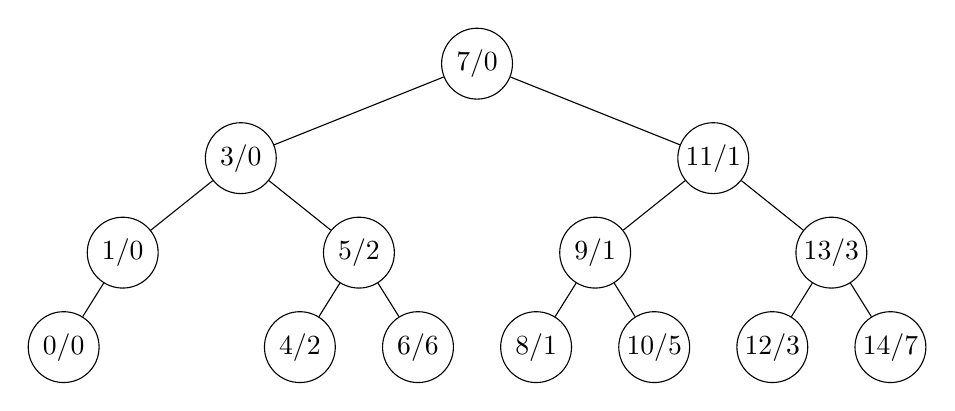
\begin{tikzpicture}[level distance=12mm,
        every node/.style={circle,draw,inner sep=0pt,minimum size=9mm},
        level 1/.style={sibling distance=60mm}, level 2/.style={sibling distance=30mm}, level 3/.style={sibling distance=15mm}]
        \node {7/0}
            child {node {3/0}
                child {node {1/0}
                    child {node {0/0}}
                    child[missing]
                }
                child {node {5/2}
                    child {node {4/2}}
                    child {node {6/6}}
                }
            }
            child {node {11/1}
                child {node {9/1}
                    child {node {8/1}}
                    child {node {10/5}}
                }
                child {node {13/3}
                    child {node {12/3}}
                    child {node {14/7}}
                }
            };
        \end{tikzpicture}
    \caption{\texttt{phase_4}的二叉树表示(节点中为参数\texttt{x}与对应返回值)}
\end{figure}

显然, 只有每层最左的节点的对应返回值为0, 符合要求. 故本关卡共有4种答案, 分别为“7 0”“3 0”“1 0”“0 0”. 输入“0 0”, 得到结果如下
\begin{code}{text}
Halfway there!
0 0

Breakpoint 4, 0x000000000040100c in phase_4 ()
(gdb) continue
Continuing.
So you got that one.  Try this one.
\end{code}

\subsection{\texttt{phase_5}}

将 \verb|phase_5| 反汇编得
\begin{code}{text}
Dump of assembler code for function phase_5:
=> 0x0000000000401062 <+0>:     push   %rbx
   0x0000000000401063 <+1>:     sub    $0x20,%rsp
   0x0000000000401067 <+5>:     mov    %rdi,%rbx
   0x000000000040106a <+8>:     mov    %fs:0x28,%rax
   0x0000000000401073 <+17>:    mov    %rax,0x18(%rsp)
   0x0000000000401078 <+22>:    xor    %eax,%eax
   0x000000000040107a <+24>:    callq  0x40131b <string_length>
   0x000000000040107f <+29>:    cmp    $0x6,%eax
   0x0000000000401082 <+32>:    je     0x4010d2 <phase_5+112>
   0x0000000000401084 <+34>:    callq  0x40143a <explode_bomb>
   0x0000000000401089 <+39>:    jmp    0x4010d2 <phase_5+112>
   ...                          ...    ...
   0x00000000004010d9 <+119>:   mov    0x18(%rsp),%rax
   0x00000000004010de <+124>:   xor    %fs:0x28,%rax
   0x00000000004010e7 <+133>:   je     0x4010ee <phase_5+140>
   0x00000000004010e9 <+135>:   callq  0x400b30 <__stack_chk_fail@plt>
   0x00000000004010ee <+140>:   add    $0x20,%rsp
   0x00000000004010f2 <+144>:   pop    %rbx
   0x00000000004010f3 <+145>:   retq
End of assembler dump.
\end{code}
注意到开头部分调用了 \verb|phase_1| 中的 \verb|string_length| 函数并与6作比较, 该关卡的有效输入应是长度为6的字符串. 难点在于段寄存器 \verb|fs| 在此处的使用. 调查发现, \verb|fs:0x28| 是GCC用于检查栈缓冲区溢出而设置的警惕标志(canary), 若函数末尾部分检查到该值发生变化, 则发生溢出, 调用 \verb|__stack_chk_fail|. 这些语句的出现说明该关卡的函数体中极有可能声明了某个字符数组并进行操作.

为了验证猜想, 继续参看省略号部分的汇编代码
\begin{code}{text}
    0x000000000040108b <+41>:    movzbl (%rbx,%rax,1),%ecx
    0x000000000040108f <+45>:    mov    %cl,(%rsp)
    0x0000000000401092 <+48>:    mov    (%rsp),%rdx
    0x0000000000401096 <+52>:    and    $0xf,%edx
    0x0000000000401099 <+55>:    movzbl 0x4024b0(%rdx),%edx
    0x00000000004010a0 <+62>:    mov    %dl,0x10(%rsp,%rax,1)
    0x00000000004010a4 <+66>:    add    $0x1,%rax
    0x00000000004010a8 <+70>:    cmp    $0x6,%rax
    0x00000000004010ac <+74>:    jne    0x40108b <phase_5+41>
    0x00000000004010ae <+76>:    movb   $0x0,0x16(%rsp)
    0x00000000004010b3 <+81>:    mov    $0x40245e,%esi
    0x00000000004010b8 <+86>:    lea    0x10(%rsp),%rdi
    0x00000000004010bd <+91>:    callq  0x401338 <strings_not_equal>
    0x00000000004010c2 <+96>:    test   %eax,%eax
    0x00000000004010c4 <+98>:    je     0x4010d9 <phase_5+119>
    0x00000000004010c6 <+100>:   callq  0x40143a <explode_bomb>
    0x00000000004010cb <+105>:   nopl   0x0(%rax,%rax,1)
    0x00000000004010d0 <+110>:   jmp    0x4010d9 <phase_5+119>
    0x00000000004010d2 <+112>:   mov    $0x0,%eax
    0x00000000004010d7 <+117>:   jmp    0x40108b <phase_5+41>
\end{code}
梳理大意如下:
\begin{enumerate}[noitemsep]
    \item 前半部分为循环结构, 依次取出输入字符数组 \verb|rbx| 中的6个字符.
    \item 每次循环, 取当前字符模16的余数为偏移量, \verb|0x4024b0| 为基地址, 从内存中取出另一字符, 存入以 \verb|rsp+10| 为首元素地址的字符数组中.
    \item 循环结束后, 调用 \verb|strings_not_equal|, 将以 \verb|rsp+10| 为首元素地址的字符数组与位于 \verb|0x40245e| 的字符串做比较, 若不相等则调用 \verb|explode_bomb|.
\end{enumerate}
此外, 还有一些与栈缓冲区溢出相关的额外处理. 根据上述逻辑, 我们只需找出字符数组 \verb|rbx| 与字符数组 \verb|rsp+10| 间各字符的映射关系, 使得字符数组 \verb|rsp+10| 的内容与 地址 \verb|0x40245e| 处的内容相同即可.

首先, 查看 \verb|0x4024b0| 的内容
\begin{code}{text}
(gdb) x/16bc 0x4024b0
0x4024b0 <array.3449>:  109 'm' 97 'a'  100 'd' 117 'u' 105 'i' 101 'e' 114 'r' 115 's'
0x4024b8 <array.3449+8>:        110 'n' 102 'f' 111 'o' 116 't' 118 'v' 98 'b'  121 'y' 108 'l'
\end{code}
可见 \verb|0x4024b0| 处实际也为字符数组, 作用域为全局.

其次, 查看 \verb|0x40245e| 的内容
\begin{code}{text}
(gdb) x/s 0x40245e
0x40245e:       "flyers"
\end{code}
知最后要求 \verb|rsp+10| 处的内容为“flyers”, 对应数组 \verb|0x4024b0| 中的下标为9, 15, 14, 5, 6, 7. 

由于映射过程中有模16运算, 本关卡的可行解较多, 此处统一取ASCII在96\textasciitilde111之间的字符, 得到一种可行解的ASCII为105, 111, 110, 101, 102, 103. 写成字符串为 "ionefg".

\begin{code}{text}
(gdb) jump *0x400ea2
Continuing at 0x400ea2.
ionefg

Breakpoint 5, 0x0000000000401062 in phase_5 ()
(gdb) continue
Continuing.
Good work!  On to the next...
\end{code}

\subsection{\texttt{phase_6}}

出于篇幅考虑, \verb|phase_6| 的完整汇编代码置于附录 \nameref{phase6}. 

该关卡的输入部分为
\begin{code}{text}
0x0000000000401100 <+12>:    mov    %rsp,%r13
0x0000000000401103 <+15>:    mov    %rsp,%rsi
0x0000000000401106 <+18>:    callq  0x40145c <read_six_numbers>
\end{code}
参照 \verb|phase_2|, 读入的6个32位整数分别位于  \verb|r13|, \verb|r13+4|, \verb|r13+8|, \verb|r13+12|, \verb|r13+16|, \verb|r13+20| 中, 往后记为 $x[i],i=0,\cdots,5$. 

随后的<+32>到<+93>是一个二重循环结构, 用C语言表达为
\begin{code}{c}
for(r12d = 0; r12d < 6; r12d++) {
    if((unsigned)([r12d] - 1) > 5) explode_bomb();
    for(ebx = r12d + 1; ebx < 6; ebx++) 
        if(x[r12d] == x[ebx]) explode_bomb();
}
\end{code}
可见要求输入的6个整数为1\textasciitilde6且互不相同.

<+108>到<+121>也是一个循环结构, 用C语言表达为
\begin{code}{c}
for(rax = r14; rax != rsi; rax += 4)
    *rax = 7 - *rax
\end{code}
注意此处 \verb|r14|, \verb|rsi| 已分别被修改为$x[0]$和$x[5]$的地址, 因此等价于$x[i] \leftarrow 7-x[i], i=0,\cdots,5$.

<+128>到<+181>也是二重循环结构, 用C语言表达为
\begin{code}{c}
for(rsi = 0; rsi != 24; rsi += 4) {
    ecx = *(x + rsi);
    if(ecx > 1){
        rdx = 0x6032d0;
        for(eax = 1; eax != ecx; eax++) rdx = *(rdx + 8);
    } else
        rdx = 0x6032d0;
    *(rsp + 32 + 2 * rsi) = rdx;
}
\end{code}
\verb|ecx|遍历了$x[0]$\textasciitilde$x[5]$的值. \verb|0x6032d0| 较为突兀, 极有可能是地址. \verb|rsp+32| 处有一数组, 每元素占8字节, 可能也是地址. 若尝试查看 \verb|0x6032d0| 处的数据
\begin{code}{text}
(gdb) x/24wx 0x6032d0
0x6032d0 <node1>:       0x0000014c      0x00000001      0x006032e0      0x00000000
0x6032e0 <node2>:       0x000000a8      0x00000002      0x006032f0      0x00000000
0x6032f0 <node3>:       0x0000039c      0x00000003      0x00603300      0x00000000
0x603300 <node4>:       0x000002b3      0x00000004      0x00603310      0x00000000
0x603310 <node5>:       0x000001dd      0x00000005      0x00603320      0x00000000
0x603320 <node6>:       0x000001bb      0x00000006      0x00000000      0x00000000
\end{code}
发现符号为 \verb|node1| \textasciitilde \verb|node6|, 可能是某种数据结构, 记“节点”为$node[i-1],i=1,\cdots,6$. 每个节点包含3个数据项, 其中第一个数据项可视作整数, 我们记为$node[i-1].data$, 第2个数据项恰为元素序号$i$, 记为$node[i-1].index$, 第3个数据项为指向$node[i]$的指针, 记为$node[i-1].next$. 那么 \verb|rdx = *(rdx + 8)| 一句等价于寻找后继节点. 我们断言地址 \verb|0x6032d0| 处存放的是单向链表, 如图 \ref{fig:list} 所示.

\begin{figure}[H]
    \centering
    \small
    \usetikzlibrary {arrows.meta}
    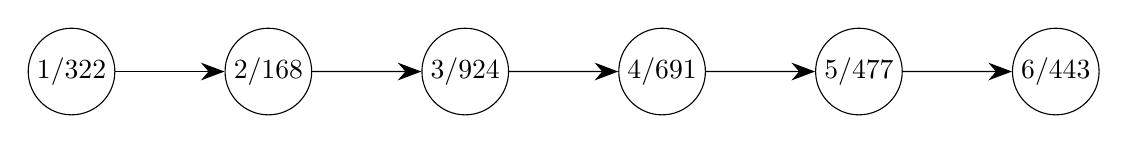
\begin{tikzpicture}[level distance=25mm,
        every node/.style={circle,draw,inner sep=0pt,minimum size=11mm},grow=right,arrows=-{Stealth[length=3mm]}]
        \node {1/322}
            child {node {2/168}
                child {node {3/924}
                    child {node {4/691}
                        child {node {5/477}
                            child {node {6/443}
                            }
                        }
                    }
                }
            };
    \end{tikzpicture}
    \caption{\texttt{phase_6}的单链表(节点中内容为“$index$/$data$”)}\label{fig:list}
\end{figure}
记数组 \verb|rsp+32| 的元素为$addr[i],i=0,\cdots,5$, 那么上述循环等价于将$addr[i]$赋值为$node[x[i]-1]$的地址. 说明输入的数据起到索引的作用.

有了上述一系列记号, <+201>\textasciitilde<+235>的循环结构可以用C语言表达为
\begin{code}{c}
node* rcx = addr;
for(node* rax = addr + 8; rax != addr + 40; rax += 8) {
    rcx -> next = rax;
    rcx = rax;
}
\end{code}
等价于$*(addr[i-1]).next \leftarrow addr[i], i=1,\cdots,5$, 使得$node[x[i-1]]$的后继节点为$node[x[i]]$

最后一个循环结构<+235>~<+257>用C语言表达为
\begin{code}{c}
node* rbx = addr;
for(ebp = 5; ebp != 0; ebp--) {
    node* rax = rbx -> next;
    if(rax -> data < rbx -> data)
        explode_bomb();
    rbx = rbx -> next;
}
\end{code}
或者说, 要求$node[x[i]] \geq node[x[i+1]]$, 否则炸弹爆炸. 

综合以上分析, 通关思路已经显然易见. 记输入的原始整数为$d[i], i=0,\cdots,5$, 那么当且仅当$node[6-d[i]].data \geq node[6-d[i+1]].data$时, 炸弹不会爆炸. 由于
$$ node[2].data < node[3].data < node[4].data < node[5].data < node[0].data < node[1].data$$
故答案为
$$d[0]=4,d[1]=3,d[2]=2,d[3]=1,d[4]=6,d[5]=5$$

输入答案, 顺利通过. 输入输出如下
\begin{code}{text}
(gdb) run
The program being debugged has been started already.
Start it from the beginning? (y or n) y
Starting program: /home/hasined/Repositories/Computer-System/labs/bomb/bomb/bomb

Breakpoint 12, printf (__fmt=<optimized out>) at /usr/include/x86_64-linux-gnu/bits/stdio2.h:105
105     printf (const char *__restrict __fmt, ...)
(gdb) jump *0x400ebe
Line 107 is not in `printf'.  Jump anyway? (y or n) y
Continuing at 0x400ebe.
4 3 2 1 6 5

Breakpoint 6, 0x00000000004010f4 in phase_6 ()
(gdb) continue
Continuing.
[Inferior 1 (process 6159) exited normally]
\end{code}

此处, 由于是直接跳转至 \verb|phase_6|, 程序并未输出通关信息.

\subsection{\texttt{secret_phase}}

为了寻找进入隐藏关卡的方法, 我们在 \verb|disas.txt| 中搜索, 发现 \verb|secret_phase| 在 \verb|phase_defused| 中被调用. 注意到汇编代码\footnote{见附录 \nameref{phase-defused}}中以下两行
\begin{code}{text}
   0x00000000004015d8 <+20>:    cmpl   $0x6,0x202181(%rip)        # 0x603760 <num_input_strings>
   0x00000000004015df <+27>:    jne    0x40163f <phase_defused+123>
\end{code}
可知当全局变量 \verb|num_input_strings| 的值为6时, 才会进行与隐藏关卡相关的判定. 进一步调查, 发现该变量在 \verb|read_line| 函数\footnote{见附录 \nameref{readline}}中被修改
\begin{code}{text}
    0x000000000040151f <+129>:   mov    0x20223b(%rip),%edx        # 0x603760 <num_input_strings>
    ...                          ...    ...
    0x000000000040155e <+192>:   mov    0x2021fc(%rip),%eax        # 0x603760 <num_input_strings>
    0x0000000000401564 <+198>:   lea    0x1(%rax),%edx
    0x0000000000401567 <+201>:   mov    %edx,0x2021f3(%rip)        # 0x603760 <num_input_strings>
    ...                          ...    ...
    0x00000000004015b3 <+277>:   add    $0x1,%edx
    0x00000000004015b6 <+280>:   mov    %edx,0x2021a4(%rip)        # 0x603760 <num_input_strings>
\end{code}
中间部分与输入过长时的错误处理有关, 此处不赘述. 由末尾部分可知, 每次读入一行字符串, 都会使 \verb|num_input_strings| 自增. 当 \verb|phase_6| 调用结束后, 应当有 \verb|num_input_strings| = 6. 验证如下
\begin{code}{text}
(gdb) break *0x4015e1
Breakpoint 13 at 0x4015e1
(gdb) run
Starting program: /home/hasined/Repositories/Computer-System/labs/bomb/bomb/bomb
Welcome to my fiendish little bomb. You have 6 phases with
which to blow yourself up. Have a nice day!
Border relations with Canada have never been better.
Phase 1 defused. How about the next one?
1 2 4 8 16 32
That's number 2.  Keep going!
0 207
Halfway there!
0 0
So you got that one.  Try this one.
ionefg
Good work!  On to the next...
4 3 2 1 6 5

Breakpoint 13, 0x00000000004015e1 in phase_defused ()
(gdb) x/w &num_input_strings
0x603760 <num_input_strings>:   6
\end{code}
发现确实在前6个关卡通过后到达了断点处. 

继续查看 \verb|phase_defused| 的汇编代码, 发现调用了 \verb|sscanf|, 以 \verb|0x402619| 为源字符串, 以 \verb|0x402619| 处的字符串为输入格式. 分别调查2个地址的内容
\begin{code}{text}
(gdb) x/s 0x402619
0x402619:       "%d %d %s"
(gdb) x/s 0x603870
0x603870 <input_strings+240>:   "0 0"
\end{code}
发现是从 \verb|input_strings+240| 读入2个整数和1个字符串. 根据符号, \verb|input_strings| 极有可能是输入字符串构成的数组. 由于 \verb|input_strings+240| 的内容与 \verb|phase_4| 的输入一致, 合理猜测, 数组为每个串分配的长度为80字节. 于是, 以 \verb|char[6][80]| 为类型查看
\begin{code}{text}
(gdb) print (char[6][80]) input_strings
$1 = {"Border relations with Canada have never been better.", '\000' <repeats 27 times>, "1 2 4 8 16 32", '\000' <repeats 66 times>,
  "0 207", '\000' <repeats 74 times>, "0 0", '\000' <repeats 76 times>, "ionefg", '\000' <repeats 73 times>,
  "4 3 2 1 6 5", '\000' <repeats 68 times>}
\end{code}
猜想得到验证. \verb|read_line| 函数每次均将输入的字符串存入全局数组 \verb|input_strings| 中. 对应到汇编代码, 主要为以下语句
\begin{code}{text}
    0x0000000000401528 <+138>:   lea    (%rax,%rax,4),%rsi
    0x000000000040152c <+142>:   shl    $0x4,%rsi
    0x0000000000401530 <+146>:   add    $0x603780,%rsi
    ...                          ...    ...
    0x0000000000401546 <+168>:   repnz scas %es:(%rdi),%al
\end{code}

总而言之, 要进入 \verb|secret_phase|, 应当在 \verb|phase_4| 输入额外的字符串. 前文提到, \verb|phase_4| 要求 \verb|sscanf| 输入数据数目严格为2, 与 \verb|phase_3| 存在微妙的区别, 已经给予了我们一定的提示.

继续查看 \verb|phase_defused| 的汇编代码, 发现调用了 \verb|strings_not_equal|, 要求输入字符串为
\begin{code}{text}
(gdb) x/s 0x402622
0x402622:       "DrEvil"
\end{code}
重新运行程序, 在 \verb|phase_4| 输入“0 0 DrEvil”, 成功来到 \verb|secret_phase| 的断点处.

\begin{code}{text}
Curses, you've found the secret phase!
But finding it and solving it are quite different...

Breakpoint 7, 0x0000000000401242 in secret_phase ()
\end{code}

反汇编得
\begin{code}{text}
    Dump of assembler code for function secret_phase:
    => 0x0000000000401242 <+0>:     push   %rbx
       0x0000000000401243 <+1>:     callq  0x40149e <read_line>
       0x0000000000401248 <+6>:     mov    $0xa,%edx
       0x000000000040124d <+11>:    mov    $0x0,%esi
       0x0000000000401252 <+16>:    mov    %rax,%rdi
       0x0000000000401255 <+19>:    callq  0x400bd0 <strtol@plt>
       0x000000000040125a <+24>:    mov    %rax,%rbx
       0x000000000040125d <+27>:    lea    -0x1(%rax),%eax
       0x0000000000401260 <+30>:    cmp    $0x3e8,%eax
       0x0000000000401265 <+35>:    jbe    0x40126c <secret_phase+42>
       0x0000000000401267 <+37>:    callq  0x40143a <explode_bomb>
       0x000000000040126c <+42>:    mov    %ebx,%esi
       0x000000000040126e <+44>:    mov    $0x6030f0,%edi
       0x0000000000401273 <+49>:    callq  0x401204 <fun7>
       0x0000000000401278 <+54>:    cmp    $0x2,%eax
       0x000000000040127b <+57>:    je     0x401282 <secret_phase+64>
       0x000000000040127d <+59>:    callq  0x40143a <explode_bomb>
       0x0000000000401282 <+64>:    mov    $0x402438,%edi
       0x0000000000401287 <+69>:    callq  0x400b10 <puts@plt>
       0x000000000040128c <+74>:    callq  0x4015c4 <phase_defused>
       0x0000000000401291 <+79>:    pop    %rbx
       0x0000000000401292 <+80>:    retq
    End of assembler dump.
\end{code}
大意如下:
\begin{enumerate}[noitemsep]
    \item 读入一行字符串, 调用标准库中 \verb|strtol| 函数将其转化为长整型.
    \item 检查输入的长整数是否小于1001, 若为否, 炸弹爆炸.
    \item 以输入的整数和 \verb|0x6030f0| 为参数, 调用 \verb|fun7| 函数. 
    \item 若 \verb|fun7| 返回值为2, 通过该关卡.
\end{enumerate}

将 \verb|fun7| 反汇编
\begin{code}{text}
Dump of assembler code for function fun7:
   0x0000000000401204 <+0>:     sub    $0x8,%rsp
   0x0000000000401208 <+4>:     test   %rdi,%rdi
   0x000000000040120b <+7>:     je     0x401238 <fun7+52>
   0x000000000040120d <+9>:     mov    (%rdi),%edx
   0x000000000040120f <+11>:    cmp    %esi,%edx
   0x0000000000401211 <+13>:    jle    0x401220 <fun7+28>
   0x0000000000401213 <+15>:    mov    0x8(%rdi),%rdi
   0x0000000000401217 <+19>:    callq  0x401204 <fun7>
   0x000000000040121c <+24>:    add    %eax,%eax
   0x000000000040121e <+26>:    jmp    0x40123d <fun7+57>
   0x0000000000401220 <+28>:    mov    $0x0,%eax
   0x0000000000401225 <+33>:    cmp    %esi,%edx
   0x0000000000401227 <+35>:    je     0x40123d <fun7+57>
   0x0000000000401229 <+37>:    mov    0x10(%rdi),%rdi
   0x000000000040122d <+41>:    callq  0x401204 <fun7>
   0x0000000000401232 <+46>:    lea    0x1(%rax,%rax,1),%eax
   0x0000000000401236 <+50>:    jmp    0x40123d <fun7+57>
   0x0000000000401238 <+52>:    mov    $0xffffffff,%eax
   0x000000000040123d <+57>:    add    $0x8,%rsp
   0x0000000000401241 <+61>:    retq
End of assembler dump.
\end{code}
发现存在递归结构, 与 \verb|func4| 极为相似. 为了帮助理解, 首先查看 \verb|0x6030f0| 附近的内容
\begin{code}{text}
(gdb) x/120wd 0x6030f0
0x6030f0 <n1>:  36      0       6304016 0
0x603100 <n1+16>:       6304048 0       0       0
0x603110 <n21>: 8       0       6304144 0
0x603120 <n21+16>:      6304080 0       0       0
0x603130 <n22>: 50      0       6304112 0
0x603140 <n22+16>:      6304176 0       0       0
0x603150 <n32>: 22      0       6304368 0
0x603160 <n32+16>:      6304304 0       0       0
0x603170 <n33>: 45      0       6304208 0
0x603180 <n33+16>:      6304400 0       0       0
0x603190 <n31>: 6       0       6304240 0
0x6031a0 <n31+16>:      6304336 0       0       0
0x6031b0 <n34>: 107     0       6304272 0
0x6031c0 <n34+16>:      6304432 0       0       0
0x6031d0 <n45>: 40      0       0       0
0x6031e0 <n45+16>:      0       0       0       0
0x6031f0 <n41>: 1       0       0       0
0x603200 <n41+16>:      0       0       0       0
0x603210 <n47>: 99      0       0       0
0x603220 <n47+16>:      0       0       0       0
0x603230 <n44>: 35      0       0       0
0x603240 <n44+16>:      0       0       0       0
0x603250 <n42>: 7       0       0       0
0x603260 <n42+16>:      0       0       0       0
0x603270 <n43>: 20      0       0       0
0x603280 <n43+16>:      0       0       0       0
0x603290 <n46>: 47      0       0       0
0x6032a0 <n46+16>:      0       0       0       0
0x6032b0 <n48>: 1001    0       0       0
0x6032c0 <n48+16>:      0       0       0       0
\end{code} 

根据符号和 \verb|phase_5| 的经验, 我们猜测这是某种数据结构, 每个节点32个字节, 共有15个节点. 每个节点$node$有3个数据项, 第1个数据项可视为整数, 记为$node.data$; 第2、3个数据项为指针, 不妨记为$node.lchild$和$node.rchild$. 种种证据暗示我们, \verb|secret_phase| 与 \verb|phase_4| 有很强的关联性. 合理猜测, 这是一棵二叉树, 符号中的数字很可能是节点所在层数以及在该层的位置. 如图 \ref{fig:tree} 所示.
\begin{figure}[H]
    \centering
    \small
    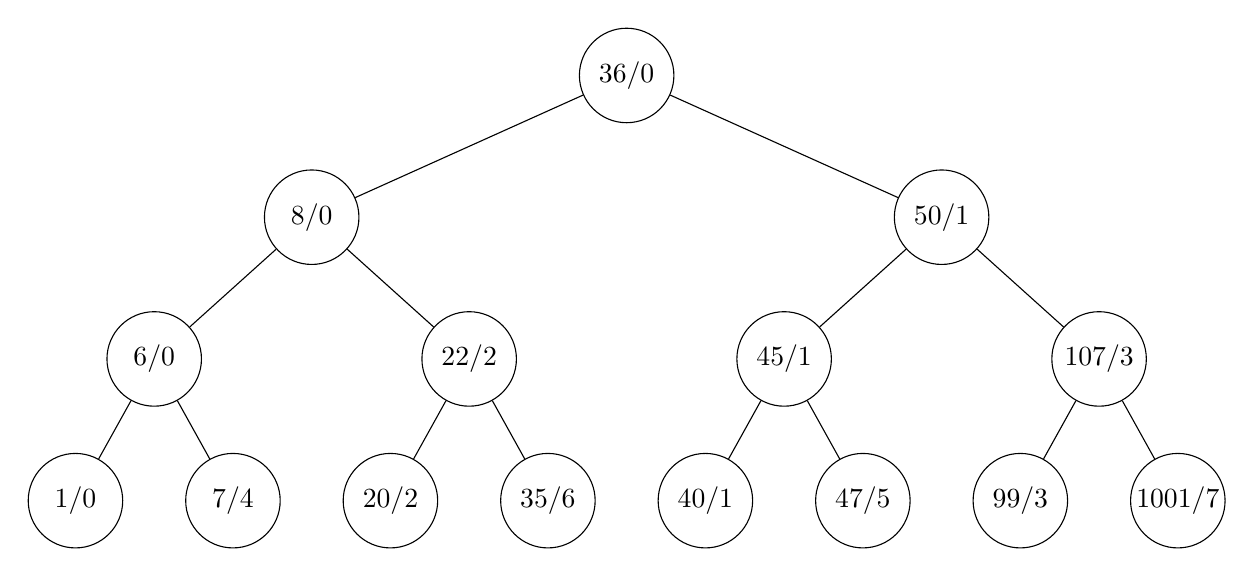
\begin{tikzpicture}[level distance=18mm,
        every node/.style={circle,draw,inner sep=0pt,minimum size=12mm},
        level 1/.style={sibling distance=80mm}, level 2/.style={sibling distance=40mm}, level 3/.style={sibling distance=20mm}]
        \node {36/0}
            child {node {8/0}
                child {node {6/0}
                    child {node {1/0}}
                    child {node {7/4}}
                }
                child {node {22/2}
                    child {node {20/2}}
                    child {node {35/6}}
                }
            }
            child {node {50/1}
                child {node {45/1}
                    child {node {40/1}}
                    child {node {47/5}}
                }
                child {node {107/3}
                    child {node {99/3}}
                    child {node {1001/7}}
                }
            };
        \end{tikzpicture}
    \caption{\texttt{secret_phase}的二叉树表示(节点中斜杠左侧内容为$node.data$)}\label{fig:tree}
\end{figure}
这是一棵二叉搜索树, 再次映证了与 \verb|phase_4| 的关联性. 于是, 可以将汇编代码翻译为
\begin{code}{c}
int fun7(int x, node* p) {
    if (!p) return -1;
    if (x < p -> data)
        return fun7(x, p -> lchild) * 2;
    else if (x > p -> data)
        return fun7(x, p -> rchild) * 2 + 1;
    else
        return 0;
}
\end{code}
发现逻辑与 \verb|phase_4| 完全一致, 仍是改写过的二分查找, 每次向左子树递归搜索, 返回值乘2; 每次向右子树递归搜索, 返回值乘2加1. 根据回溯过程, 若成功查找到 \verb|x|, 则返回值如图 \ref{fig:tree} 节点中斜杠右侧所示; 若未查找到 \verb|x|, 返回负值.

要求返回值为2, 故答案为20或22.
\begin{code}{text}
(gdb) continue
Continuing.
22
Wow! You've defused the secret stage!
Congratulations! You've defused the bomb!
[Inferior 1 (process 6228) exited normally]
\end{code}

\clearpage
\section{总结}

完成Bomb Lab, 主要有以下收获:

\begin{itemize}
    \item 提高了阅读x86-64汇编代码的能力, 加深了对函数调用、参数传递的理解.
    \item 理解了GCC中 \verb|for|、 \verb|switch|、负数除2、乘80等语句的编译方式, 认识到编译器的优化对性能的重要性. 
    \item 熟悉了链表、二叉树等数据结构的汇编表达.
    \item 学会了在终端中使用gdb调试汇编程序, 掌握了基本的反汇编、逆向工程方法.
    \item 学会了GNU Binutils中的实用命令, 借此理解了ELF文件的构造, 程序头、节头、符号表、程序段、数据段等概念.
    \item 理解了编译器对栈缓冲区溢出提供保护的方式.
    \item 认识到Docker容器和QEMU的局限性.
    \item 学会了在 \LaTeX 中使用 \verb|tikz| 宏包绘图.
\end{itemize}

本实验的所有材料已上传至GitHub:

\url{https://github.com/HasiNed/Computer-System}

\setupappendix

\clearpage
\section{部分输出结果}

\subsection{\texttt{syms.txt}}\label{syms}

\includecode{text}{syms.txt}

\subsection{\texttt{rodata.txt}}\label{rodata}

\includecode{text}{rodata.txt}

\subsection{\texttt{strings_not_equal.txt}}\label{strings-not-equal}

\includecode{text}{strings-not-equal.txt}

\subsection{\texttt{read_six_numbers.txt}}\label{read-six-numbers}

\includecode{text}{read-six-numbers.txt}

\subsection{\texttt{func4.txt}}\label{func4}

\includecode{text}{func4.txt}

\subsection{\texttt{phase_6.txt}}\label{phase6}

\includecode{text}{phase-6.txt}

\subsection{\texttt{phase_defused.txt}}\label{phase-defused}

\includecode{text}{phase-defused.txt}

\subsection{\texttt{read_line.txt}}\label{readline}

\includecode{text}{read-line.txt}